\section{A Refactored Version of the TPPSM}
\label{sec:refactored_TPPSM}
After carefully analyzing the publicly available codes implementing the TPPSM, developed by the Satellite Navigation and Sensing Lab at the University of Colorado Boulder \cite{githubGitHubCusenselabgnssscintillationsimulator} \cite{githubGitHubCusenselabgnssscintillationsimulator_2param}, it became evident that a new implementation was necessary. The existing codes did not simultaneously support simulations in the weak scattering regime and the use of real satellite orbits, making it impossible to study both conditions together. Additionally, a significant lack of documentation was observed across several functions, and some portions of the code were unorganized.

To address these limitations, a refactored version of the TPPSM was developed, using the previous codes as references. The reader can access it in \cite{githubGitHubRodrigodelimafgnssscintillationsimulator}. The validation of this refactored version is performed herein by comparing the intensity and phase spectra of a simulated scintillation time series with their theoretical counterparts, computed using a C code developed for a comprehensive analysis of the two-component power-law model \cite{Carrano2016OverviewOfTwoComponentPowerLaw}.

The simulations were conducted using the following parameters: the date and time were set to 2024/01/02 at 10:00:00 (UTC), with the receiver located in Hong Kong at a latitude of $22.21^\circ$, a longitude of $114.28^\circ$ and height of 59.6780 m. The satellite used was PRN 18, and the mean zonal drift velocity was 100 m/s. The receiver was assumed to be static, and the proposed irregularity parameter set presented in Section \ref{subsec:common_values_irr_param} was applied.

Figure \ref{fig:sdfs} illustrate the spectral comparisons for different scintillation severity cases and GPS frequency bands, namely L1, L2, and L5, using the same seed for each realization. The results show excellent agreement between the spectra generated by the refactored code and the theoretical values for both intensity and phase spectra across all cases. Here, the pre-propagation field refers to the complex field expression: $\exp\left\{ j \overline{\phi} \left[ m \right] \right\}$ whereas the post-propagated field is related to Equation \eqref{eq:post-prop_scint_field}. Notably, the post-propagated scintillation field exhibits distortions in the high-frequency portion of its spectrum. This effect clearly demonstrates the phase distortions caused by free-space propagation at the receiver plane, which directly contributes to the occurrence of cycle slips and rapid phase oscillations, potentially leading to tracking loop instabilities.
\begin{figure*}[ht]
    \centering
    \begin{subfigure}[b]{\textwidth}
        \centering
        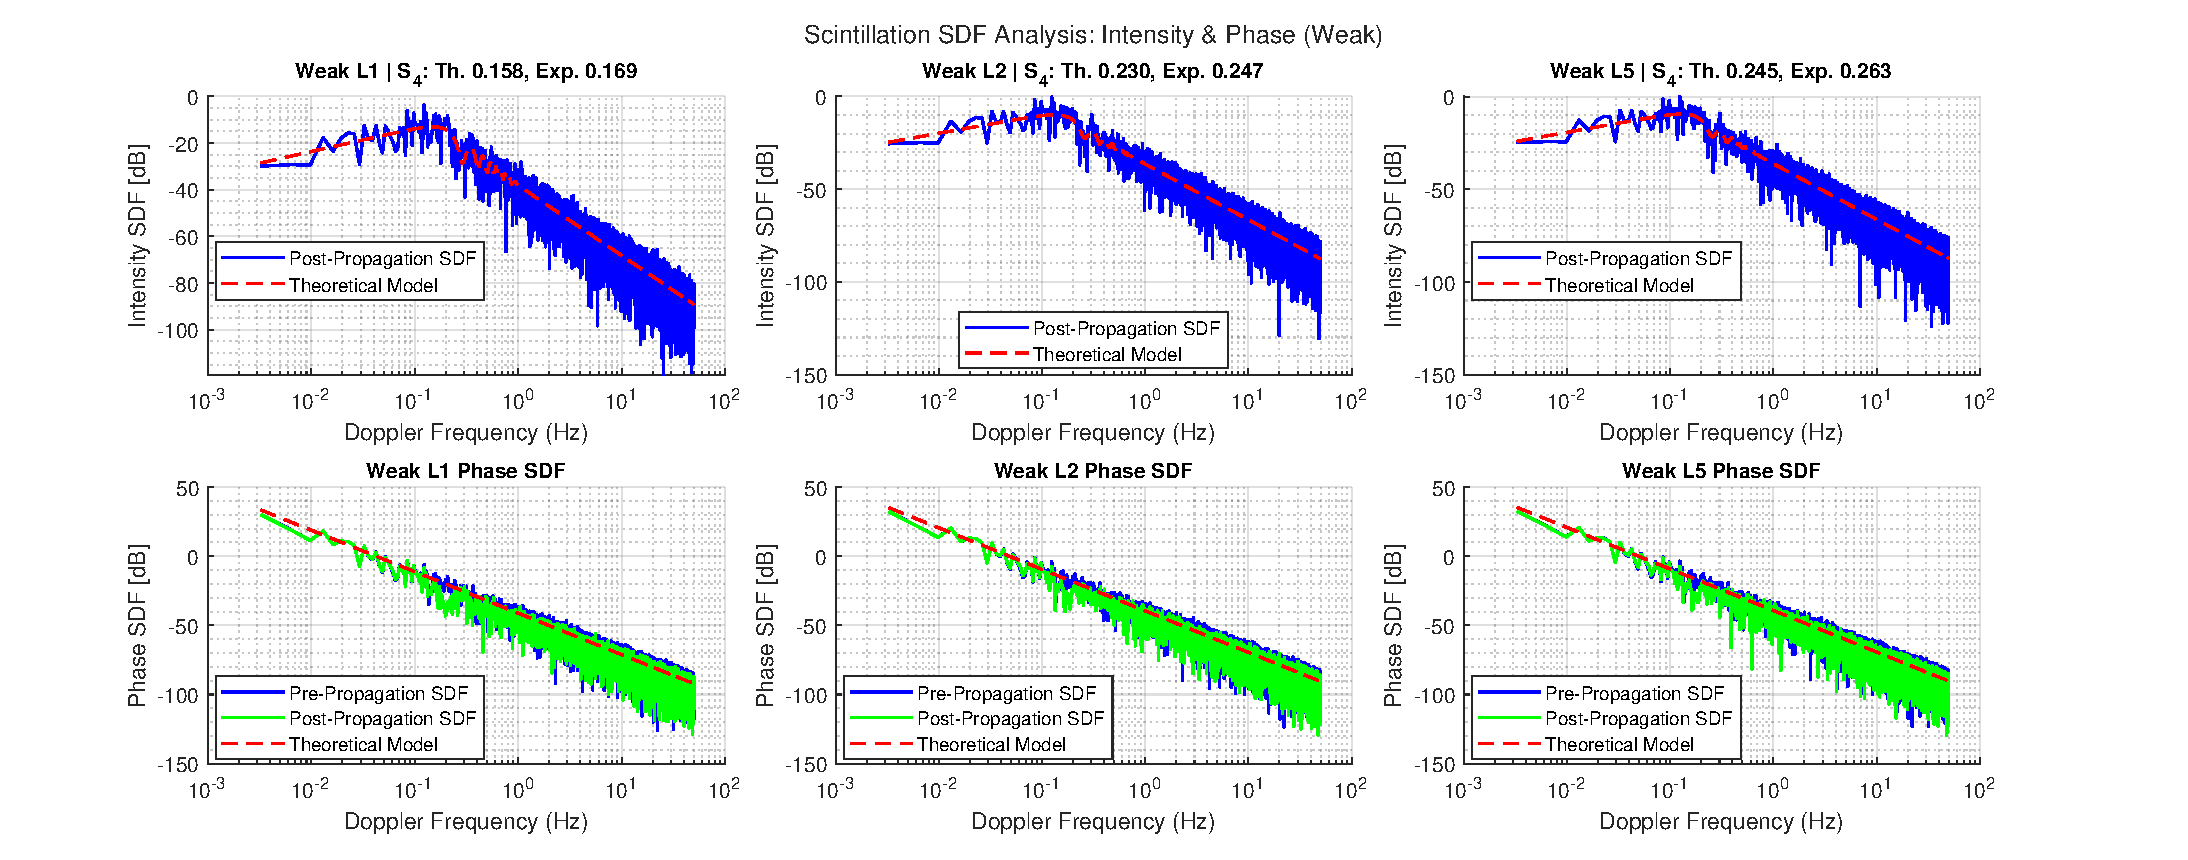
\includegraphics[width=\textwidth]{Weak_Scintillation_SDFs.pdf}
    \end{subfigure}
    \vspace{10pt} % Adjusts spacing between figures
    \begin{subfigure}[b]{\textwidth}
        \centering
        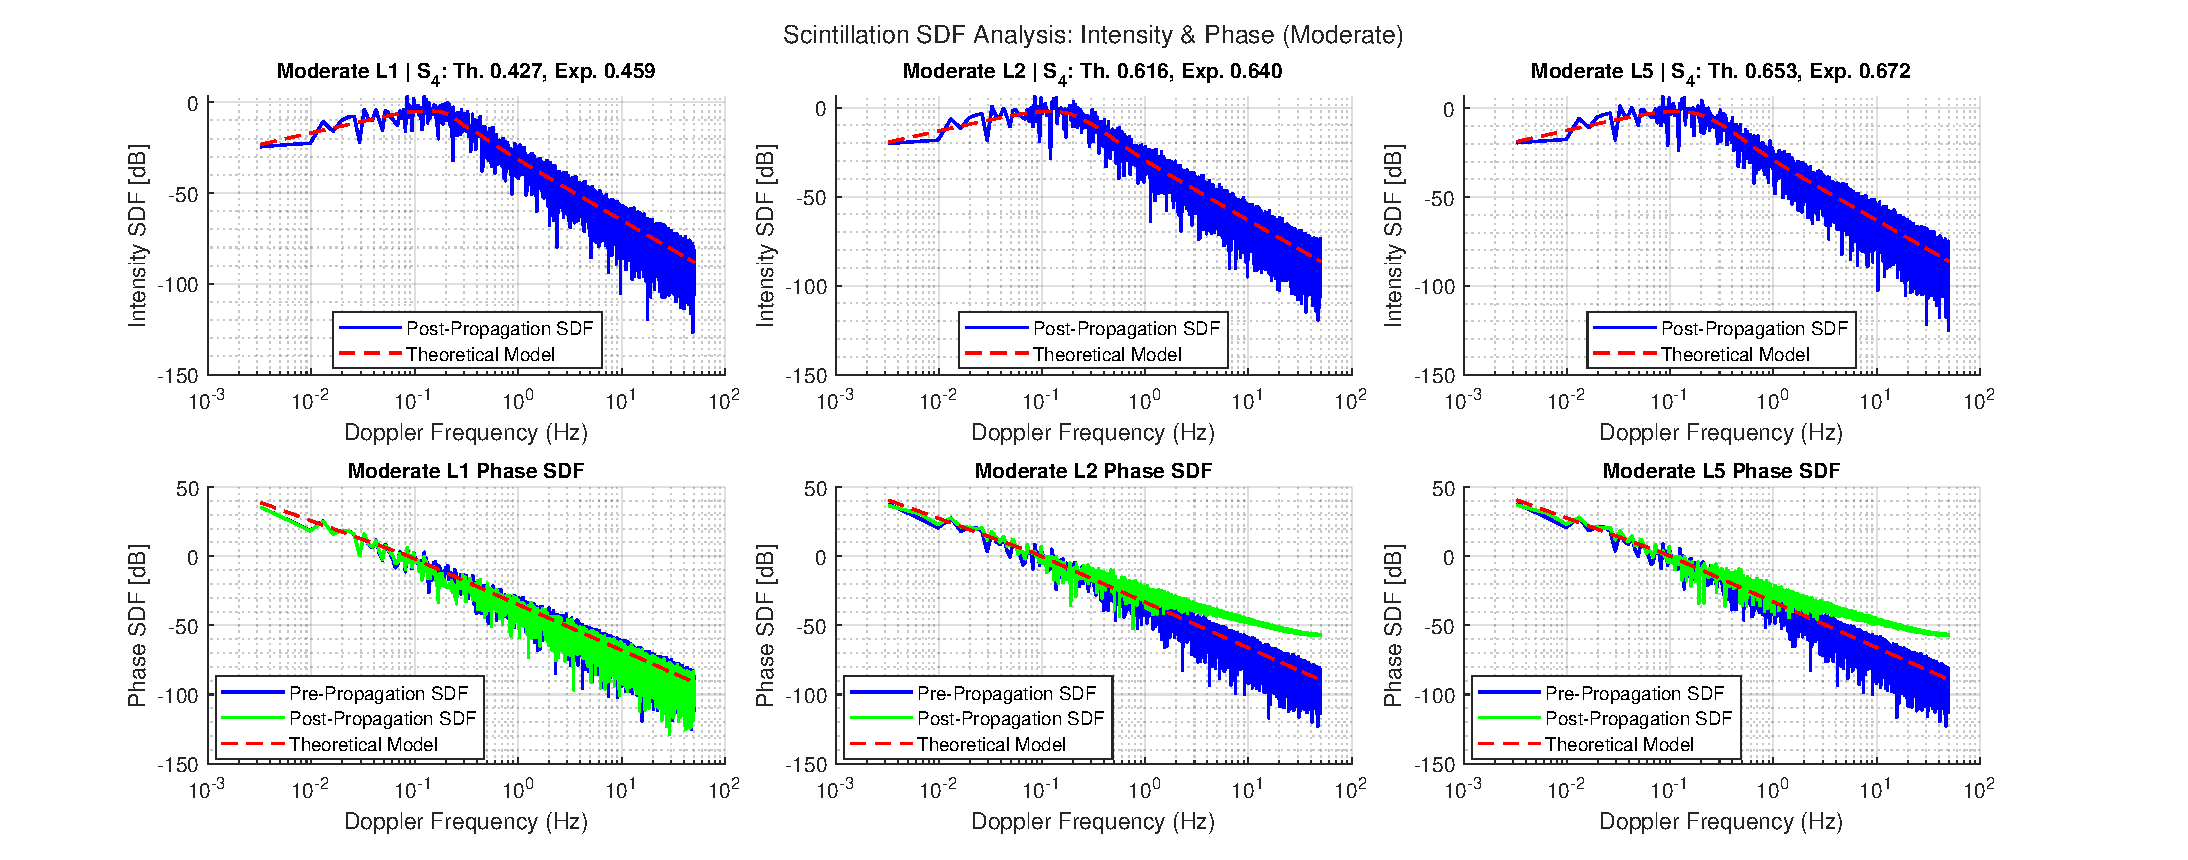
\includegraphics[width=\textwidth]{Moderate_Scintillation_SDFs.pdf}
    \end{subfigure}
    \vspace{10pt} % Adjusts spacing between figures
    \begin{subfigure}[b]{\textwidth}
        \centering
        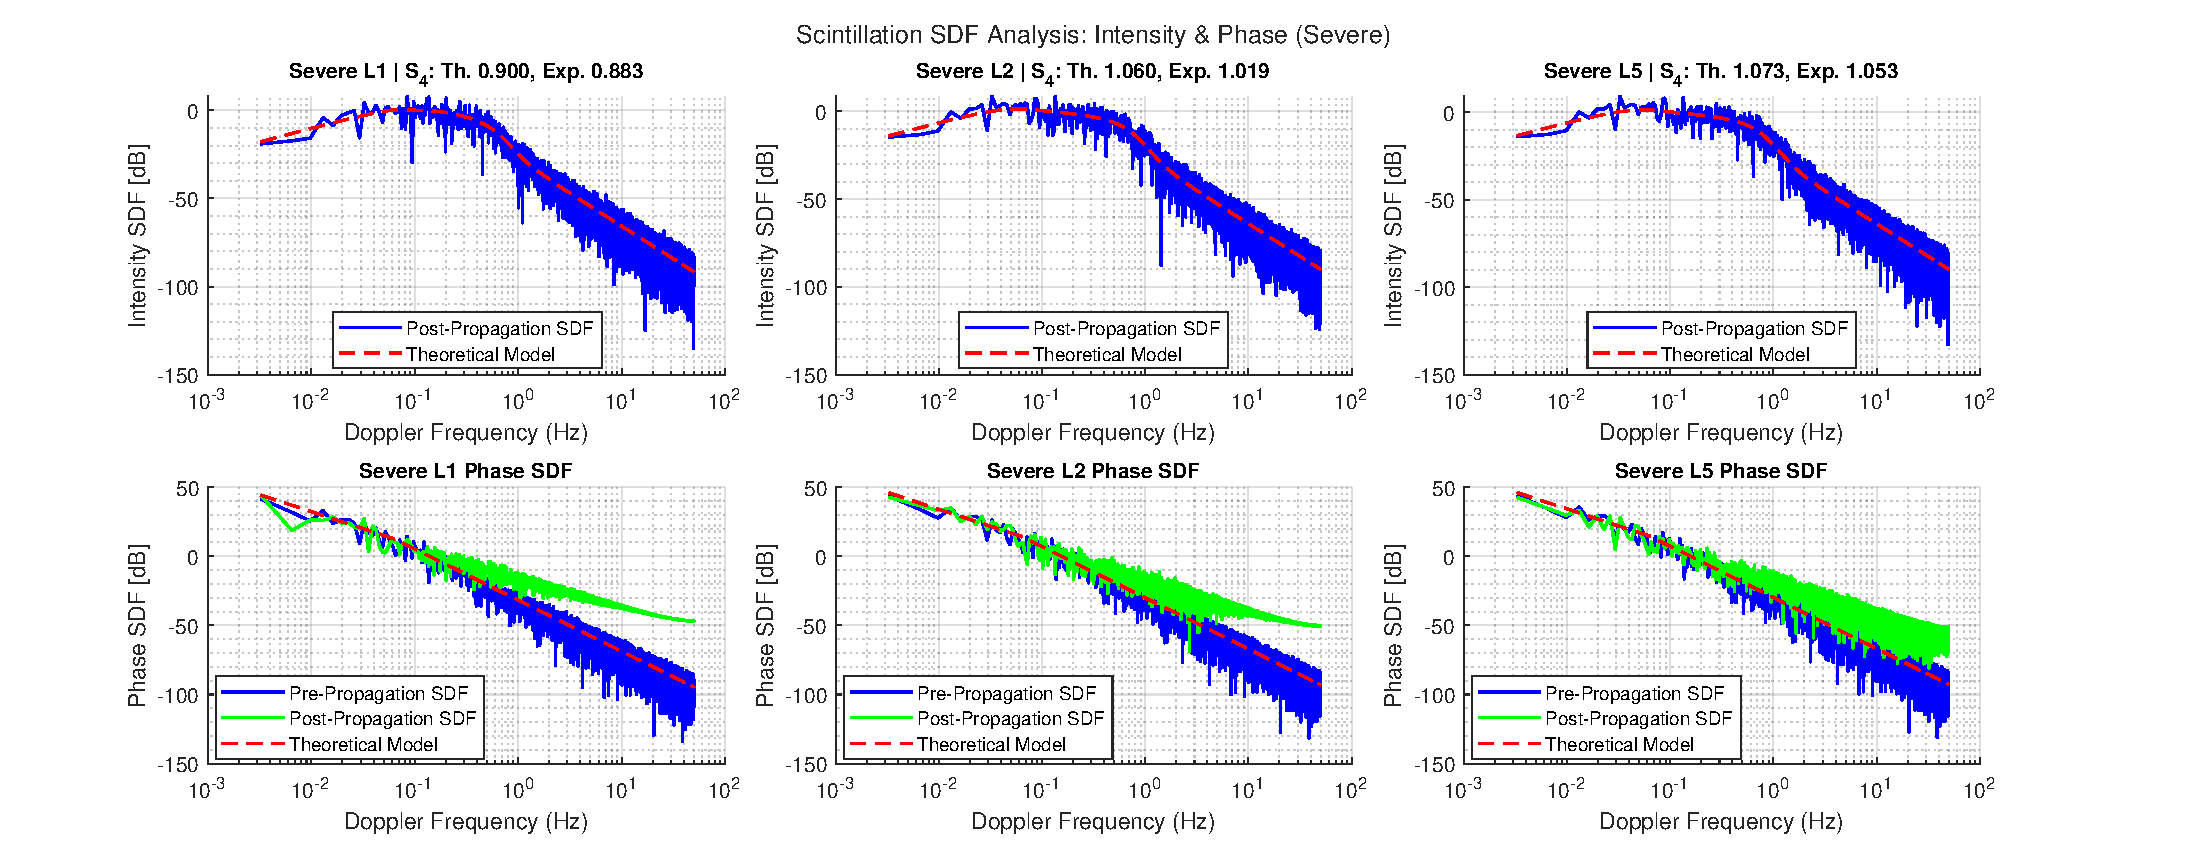
\includegraphics[width=\textwidth]{Severe_Scintillation_SDFs.pdf}
    \end{subfigure}
    \caption{This figure presents a comparison of spectral density functions (SDFs) for intensity and phase scintillation across three different severity levels: Severe, Moderate, and Weak. The analysis is performed for GPS L1, L2, and L5 frequency bands, arranged in a $2 \times 3$ grid for each severity case. The top row displays the Intensity SDF, where the blue line represents the post-propagation scintillation spectrum and the red dashed line corresponds to the theoretical intensity spectrum. The bottom row illustrates the Phase SDF, with the blue line showing the pre-propagation phase SDF, the green line indicating the post-propagation phase SDF, and the red dashed line representing the theoretical phase spectrum. The Severe case exhibits stronger spectral power and increased distortions, with significant deviations at high frequencies in the phase spectrum. The Moderate case presents an intermediate spectral behavior, while the Weak case follows the expected power-law trend with minimal deviations. These results highlight the impact of different scintillation severity levels on the signal’s intensity and phase, particularly emphasizing phase distortions in the post-propagation spectrum, which can lead to cycle slips and rapid phase oscillations, potentially affecting GNSS tracking loops. It is important to underpin that the experimental value of $S_4$ presents a statistical variability, which explains the slight discrepance of theoretical value. For further details on how these plots were obtained, please refer to \cite{githubGitHubRodrigodelimafgnssscintillationsimulator}}
    \label{fig:sdfs}
\end{figure*}

Furthermore, Figure \ref{fig:timeseries} present examples of the magnitude and phase time series of the propagated scintillation field for each scintillation severity level and frequency band considered for GPS applications. Although the current implementation only supports the L1, L2, and L5 GPS frequency bands, it can be easily modified to accommodate any GNSS frequency band.

Another noteworthy limitation of the simulator is that it currently only supports receivers moving in a rectilinear trajectory. To extend its capabilities, modifications would be required to allow the generation of scintillation time series for receivers with arbitrary trajectories. This enhancement would be particularly valuable for simulating scintillation effects on rockets, aircraft, and drone trajectories, among others.

\begin{figure*}[ht]
    \centering
    \begin{subfigure}[b]{\textwidth}
        \centering
        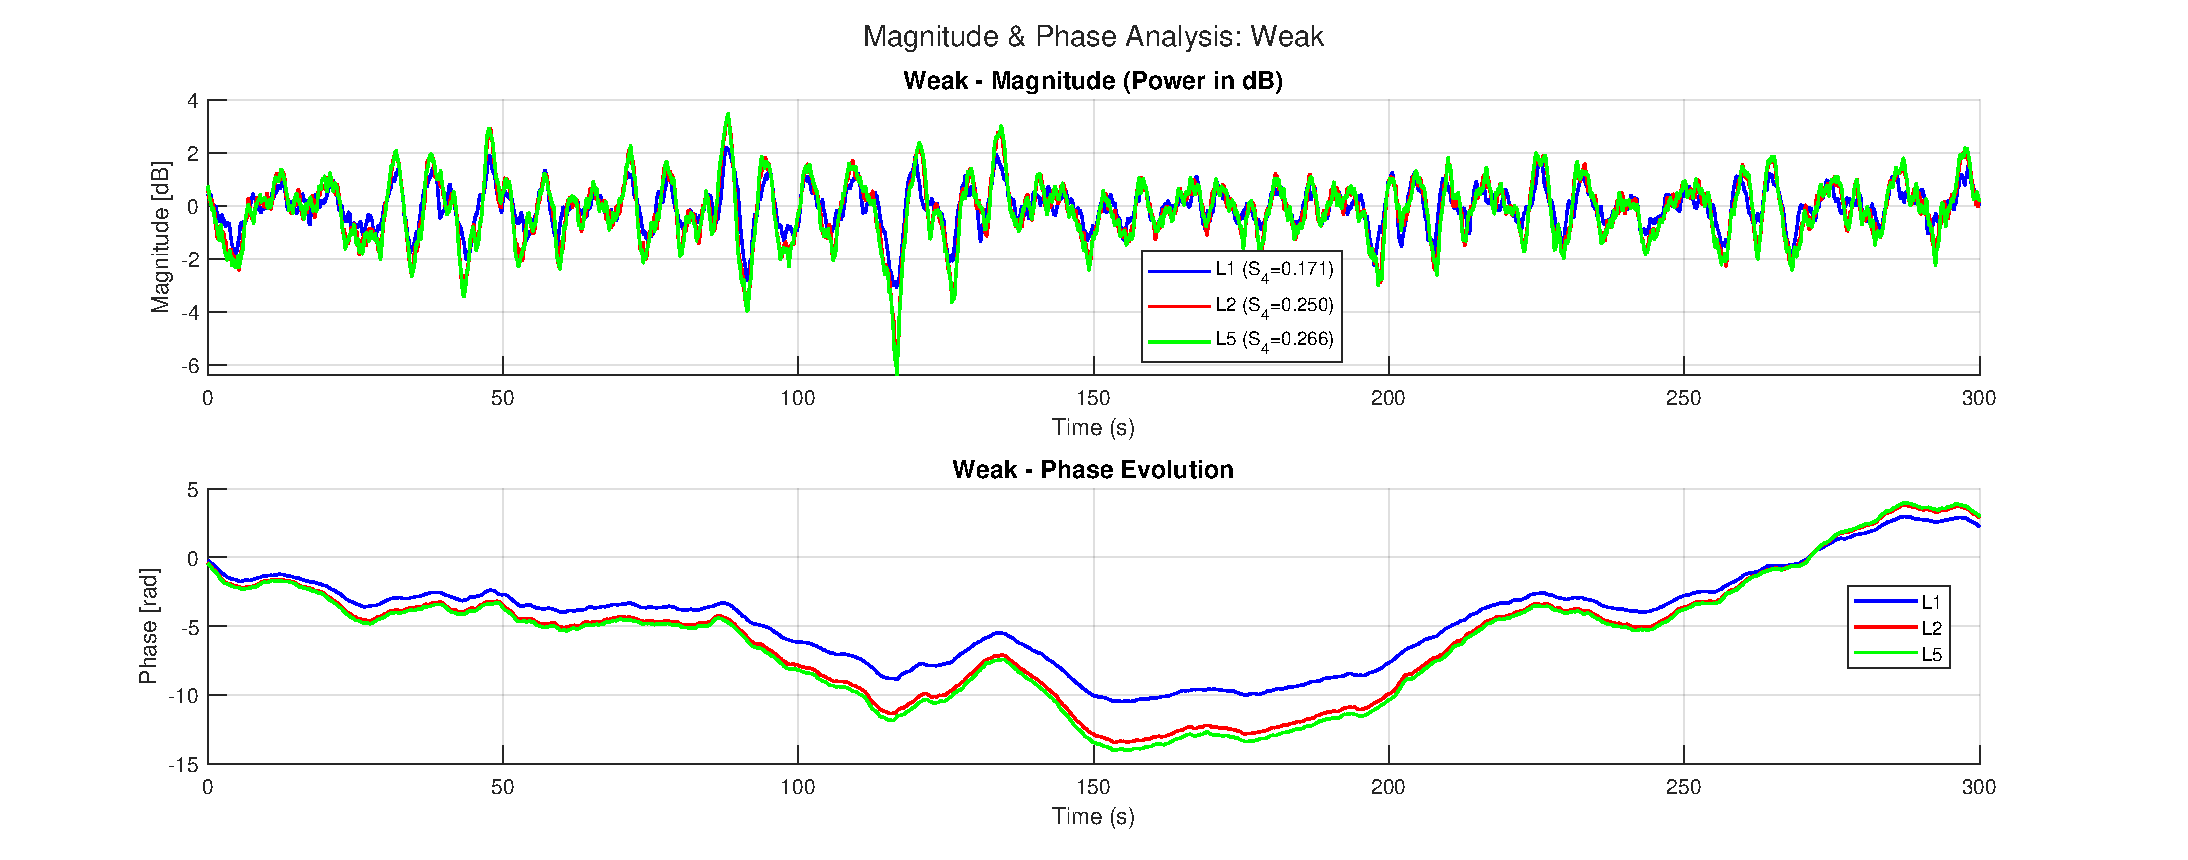
\includegraphics[width=\textwidth]{Weak_Magnitude_Phase_Time_Series.pdf}
    \end{subfigure}
    \vspace{10pt} % Adjusts spacing between figures
    \begin{subfigure}[b]{\textwidth}
        \centering
        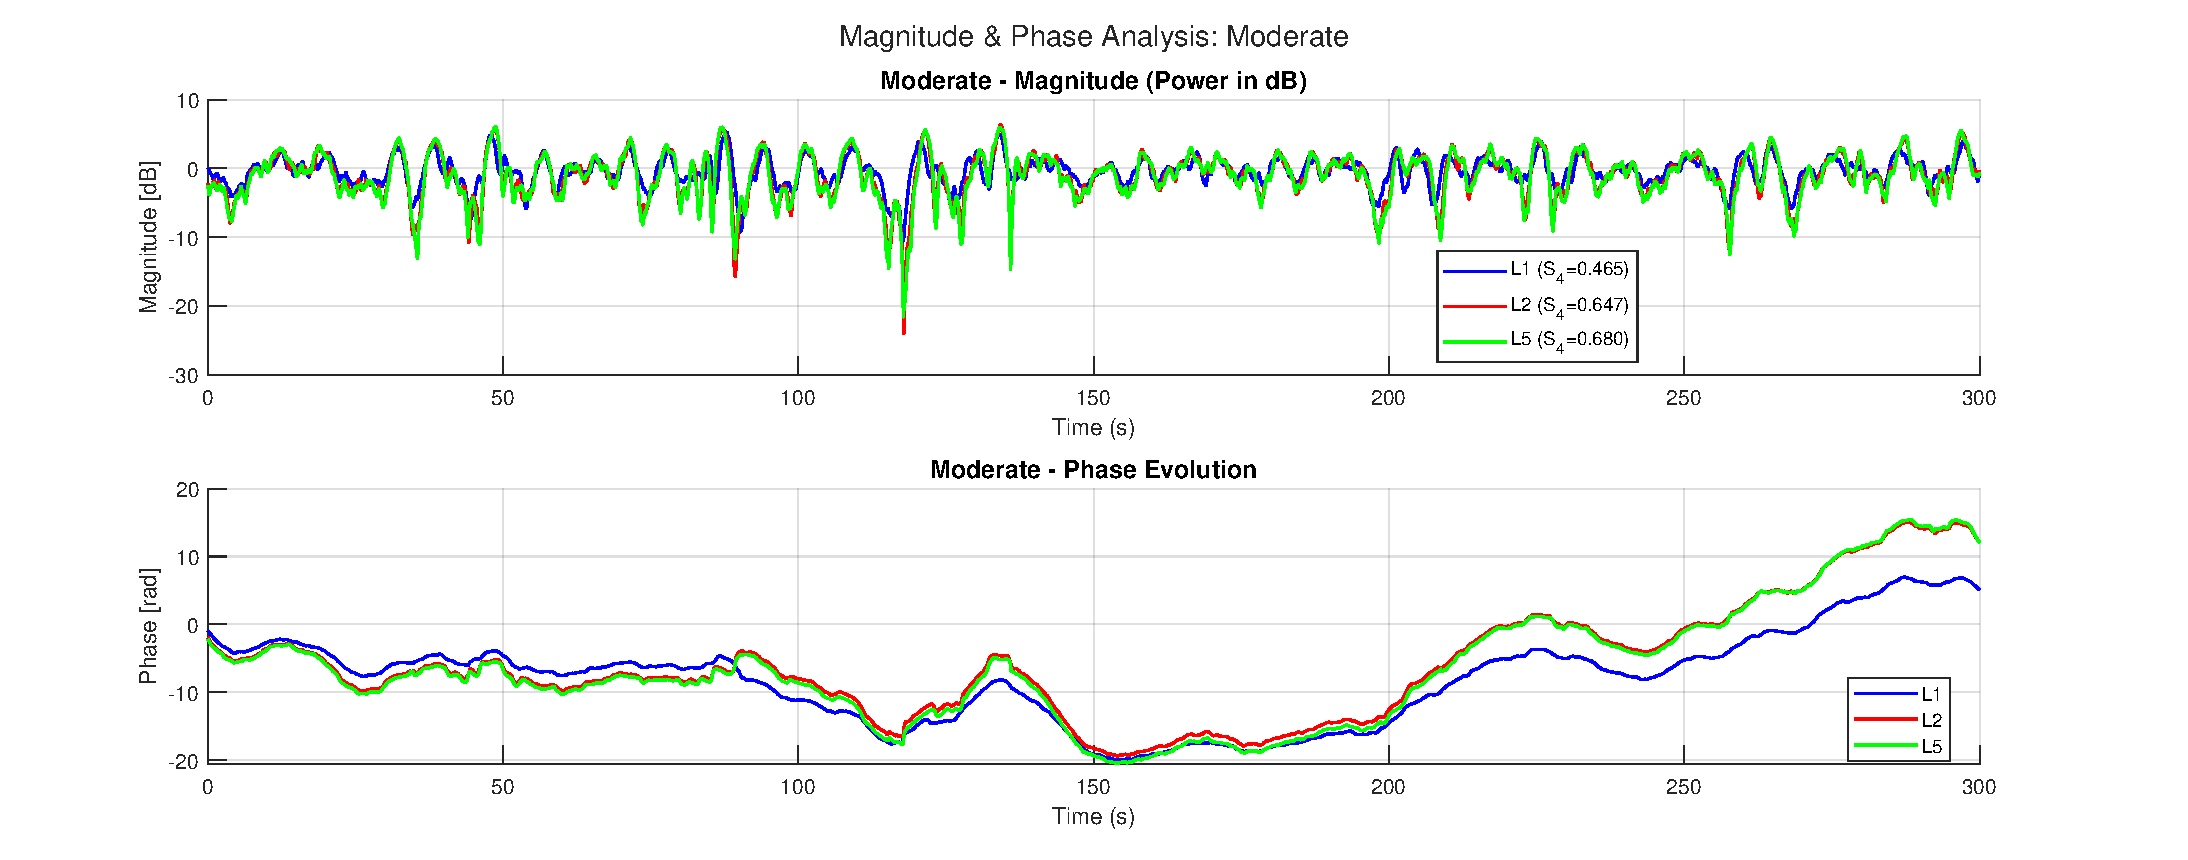
\includegraphics[width=\textwidth]{Moderate_Magnitude_Phase_Time_Series.pdf}
    \end{subfigure}
    \vspace{10pt} % Adjusts spacing between figures
    \begin{subfigure}[b]{\textwidth}
        \centering
        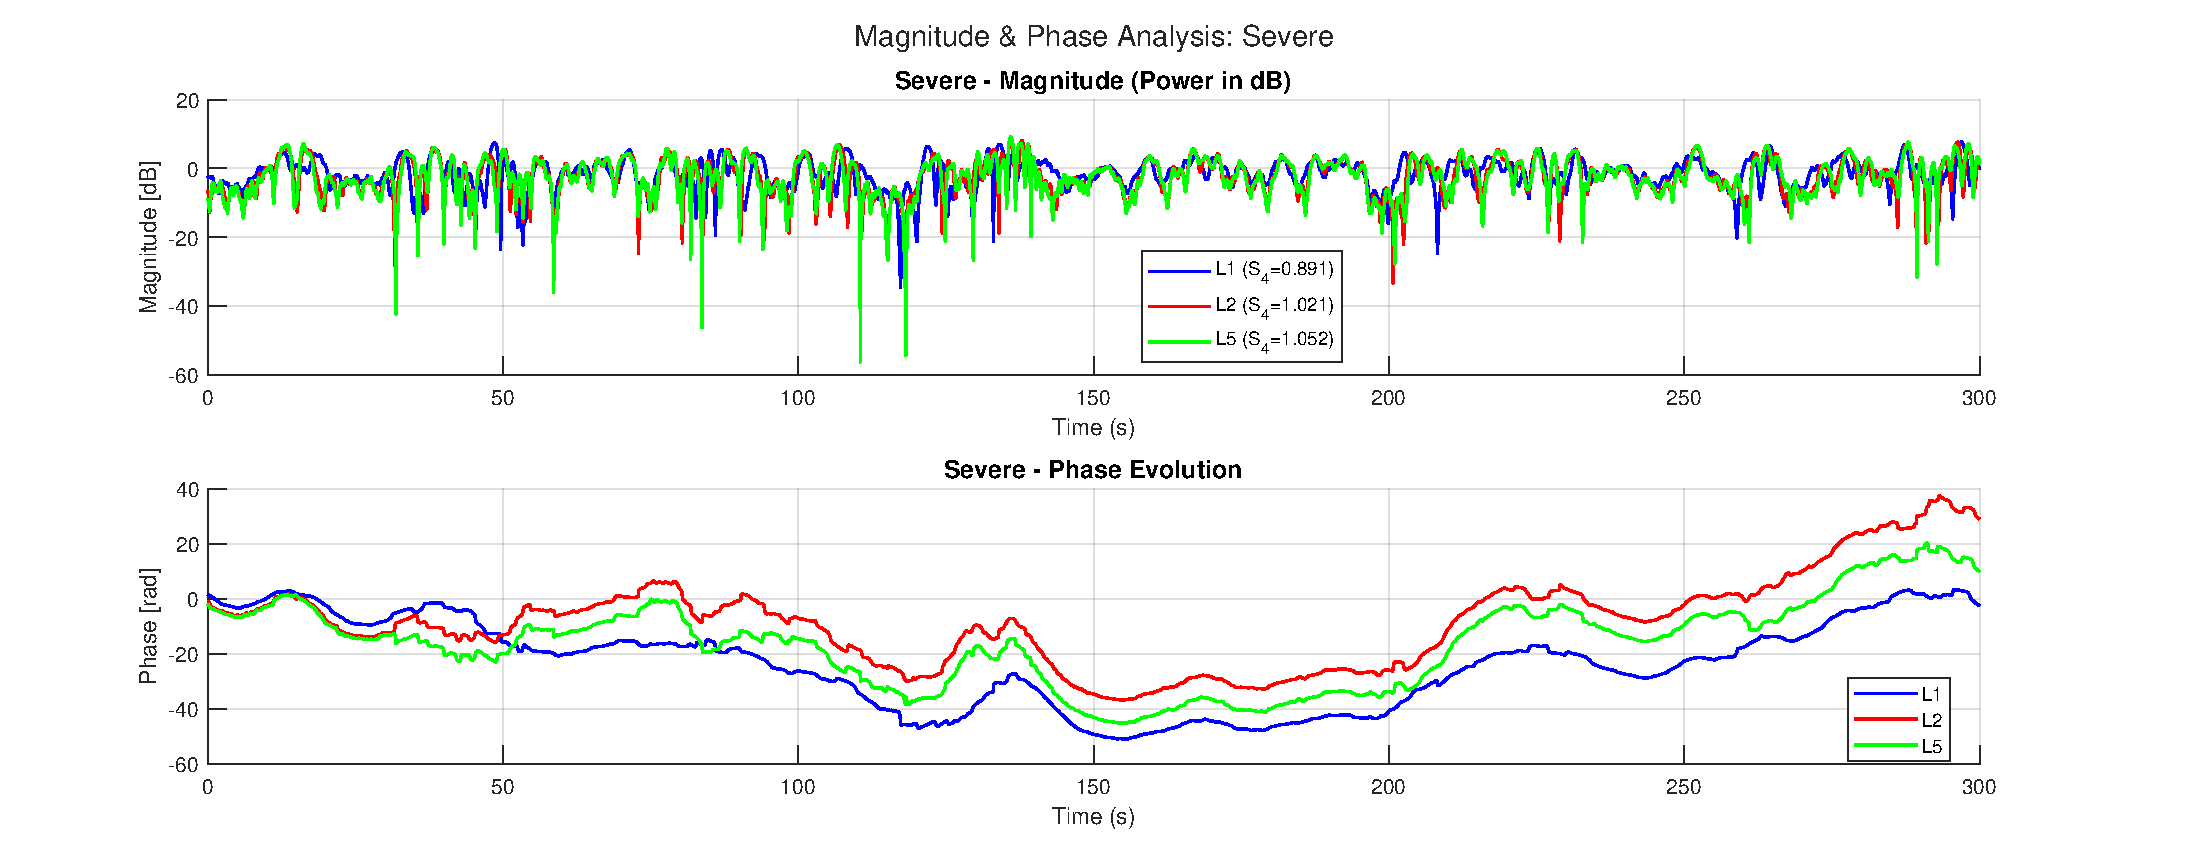
\includegraphics[width=\textwidth]{Severe_Magnitude_Phase_Time_Series.pdf}
    \end{subfigure}
    \caption{This figure presents the time series of signal magnitude (top row) and phase evolution (bottom row) for GPS L1, L2, and L5 frequency bands under different scintillation conditions: Severe, Moderate, and Weak. The magnitude is shown in dB as $10\log_{10}{\lvert \psi\left[ \rho_F; m \right]^{2} \rvert}$, while the phase in radians is computed as an unwrapped version of 2 quadrant arctangent of the imaginary and real parts of $\psi\left[ \rho_F; m \right]$. The colors represent different frequencies: blue (L1), red (L2), and green (L5). The top row illustrates the power fluctuations of the scintillation-affected signal, where higher scintillation severity leads to stronger amplitude fading. The bottom row shows the phase evolution, where increased scintillation severity causes larger phase variations, which may lead to cycle slips and phase tracking difficulties in GNSS receivers. The computed $S_4$ indices, displayed in the legend, quantify the scintillation strength for each frequency band. For further details on how these plots were obtained, please refer to \cite{githubGitHubRodrigodelimafgnssscintillationsimulator}}
    \label{fig:timeseries}
\end{figure*}
